%+
% SECTION:
%    supernovacosmology.tex
%
% CHAPTER:
%    cosmology.tex
%
% ELEVATOR PITCH:
%    SNIa cosmology, approach to evaluating dependence of science on cadence
%
%-
% ====================================================================
\clearpage
\section{Supernova Cosmology and Physics}
\def\secname{supernovae}\label{sec:\secname}

\newcommand{\ml}[1]{\textcolor{red}{[{\bf ML}: #1]}}

Lead authors:
\credit{jhrlsst},
\credit{rbiswas4},
\credit{MichelleLochner}

Contributing authors:
\credit{sethdigel},
\credit{RobFirth},
\credit{astrofoley},
\credit{lgalbany},
\credit{pgris},
\credit{ReneeHlozek},
\credit{ivezic},
\credit{saurabhwjha},
\credit{RickKessler},
\credit{AlexGKim},
\credit{aimalz},
\credit{jasonmcewen},
\credit{janewman-pitt-edu},
\credit{hiranyapeiris},
\credit{kponder},
\credit{rlschuhmann},
\credit{astrostubbs},
\credit{msullivan318},
\credit{wmwv}

\subsection{Introduction}
The acceleration of the rate of expansion of the Universe at late times is one of the
most exciting and fundamental discoveries\citep{Riess1998,Perlmutter1999} in recent times.
This discovery was made using Type Ia supernovae (SNIa) as standardizable candles, and
implies that 76\% of the energy density of the Universe is composed of dark energy
\citep{Frieman2008}. Type Ia supernovae are believed to be explosions of white
dwarfs that have approached the Chandrasekhar mass and are disrupted by
thermonuclear fusion of carbon and oxygen.


This section is concerned with the detection and characterization of
supernovae (SNe) over time with LSST and their various scientific
applications. A crucial application is the use of SNIA %and potentially some core-collapse SNe
(like type IIP) to trace
to trace the recent expansion history of the universe, and confront models of the
physics driving the late time accelerated expansion of the universe.

LSST will improve on past surveys by observing a substantial number of well-characterized
supernovae, at high redshift. This large sample is not necessarily tied to the large area of LSST
and can rather be obtained from a relatively small spatial region, such as the Deep Drilling Fields
(DDF) with larger numbers of well-measured light curves due to the long time interval and high volume
at high redshifts.

On the other hand, the Wide-Fast-Deep (WFD) aspect will make the LSST survey
the first to scan a very large area of the sky for SNe. SNe that are detected
and well characterized by the WFD will provide 
\begin{itemize}
    \item a large, well-calibrated low redshift sample ($z \lesssim 0.1$) to replace/supplement the current  set of low redshift supernovae from a mixture of surveys. Such a large, clean low redshift sample is crucial in {\emph{providing a longer lever arm for the determination of cosmological parameters from supernovae.}}
    \item  a low and medium redshift ($z \lesssim 0.8$ and peaking at $z \sim 0.4$ ) sample spanning large areas of 
the sky and therefore with the ability of {\emph{tracing large scale structure}} in a novel way, particularly due to 
the inclusion of estimates radial distances. This will be possible by combining redshift estimates from supernova light 
curves in conjunction with photometric redshifts from host galaxies.  Such a sample could also be used to probe the 
{\emph{isotropy of the late time universe.}}
    \item This large sample of SNe will also enable further sharpening of our understanding of the properties of the SN population of both Type Ia and core-collapse SNe (see \autoref{sec:transients:SNtransients}). Aside from the science described in \autoref{sec:transients:SNtransients}, this understanding will also be extremely important to the goal of SN cosmology from LSST. When selecting supernovae satisfying specific criteria from observations in magnitude limited surveys, a lack of understanding of the population properties leads to selection biases in SNIa cosmology as well as the steps in photometric classification~\cite{2017ApJ...836...56K,2016ApJ...822L..35S}. 
The WFD SN Ia
sample will dramatically increase the size of the sample available to
train such an empirical model, as well as understand the probability of
deviations and scatter from this model. Aside from issues like
calibration which need to be addressed separately, a larger sample of
such well measured SNe is probably the only way to address `systematics'
due to deviations from the empirical model. 
\end{itemize}
%The anticipated WFD sample can
%be thought of as consisting of two components:  the low-redshift sample
%which is more likely to be complete, and the higher-redshift sample that
%will be able to constrain evolution.

% --------------------------------------------------------------------

\subsection{Target measurements and discoveries}
\label{sec:\secname:targets}

SNe of different types are visible over observer time scales of about a few
weeks (e.g., type Ia) to nearly a year (type IIP).  During the full
ten-year survey, LSST will scan the entire southern sky repeatedly with
a WFD cadence, and certain specific locations of the sky called the Deep
Drilling Fields (DDF) with special enhanced cadence.

This spatio-temporal window should contain millions
of SNe. However, the actual sequence of
observations by LSST, defined by the series of field pointing as a
function of time in filter bands (along with weather conditions), and
conditions used for detection will determine the extent to which each
SN can be detected and characterized well.  Characterization of the SNe
is at the core of a number of science
programs that use them as bright, abundant objects with empirically
determined intrinsic brightnesses. While type IIP supernovae may prove to be useful standard
candles \citep{Sanders2014}, we will focus this work on the more well-established type Ia SNe.

Ultimately, the study of dark energy using LSST supernovae will be performed by an analysis inferring the parameters of a cosmological model using a sample of supernovae constructed from the LSST observations, and astrophysical models of supernovae that allow one to relate the peak intrinsic brightness to observed properties of the supernova. We should emphasize that while such analyses have been performed on previous SN surveys, the analyses that would be performed on a really large dataset would be different and is currently under study. Estimates of the potential of such surveys have often been measured using figures of merit such as the Dark Energy Task Force figure of merit~\citep{Albrecht2006}. The main goal of such a metric is to estimate the potential of a survey in elucidating the understanding of dark energy. However, our primary aim here is to study the relative impact that different LSST Observing strategies would have on such dark energy analysis, rather than absolute impact, and to communicate the characteristics of the survey that make a strategy better than others. This necessitates studying the quality of observations corresponding to typical individual supernovae or groups of supernovae rather than producing a single output for a survey. Therefore we identify some of the key steps in the supernova analysis which are directly related to observational characteristics of survey, and define metrics in terms of such quantities. In fact, these metrics should be  thought of as a total of scores, where these scores characterize the sequences of observation on small patches of the sky in small time windows. The key steps we have chosen are
\begin{enumerate}
\renewcommand{\theenumi}{\alph{enumi}}
\item The detection of SNe \label{it:detection}
\item Estimating the intrinsic peak brightness of a supernovae and its redshift
\item Photometric classification \label{it:typing}
\end{enumerate}
The efficacy of photometric typing, redshifts and estimation of intrinsic brightnesses
are all dependent on the amount of information available in the observed
light curves of SNe. While these steps are not necessarily independent, it
is useful to think of the requirements on some of these steps separately;
it is not unlikely  that combinations of some of the steps would still be
affected by similar requirements. Further, in the absence of a complete analysis, we opt for certain ad-hoc criteria in determining the threshold for such observations. This would be necessary even if we were to perform an analysis similar to past surveys.

{\emph{Supernova detection}}\\
Supernova light curves consisting of flux measurements at different times are built through photometry
at specific locations on each of the observed images. A finite list of such specific locations is
constructed through a transient detection pipeline studying difference images. In brief, this process
consists of studying subtractions between a  `template' image (coadded over time so that a supernova
flux averages to a small value) and single visit images called `science images' at different times,
after correcting for differences in resolution, observing conditions and pixel registration. In such
difference images, one expects to obtain non zero pixel values at locations of transients including
supernovae, and pixel values at other locations (including locations of static astrophysical
sources) to be
consistent with zero aside from noise. The efficiency of detecting a supernova in a single
exposure
depends on a number of factors, the most significant of which is the signal (brightness of the supernova
in the science image compared to the template) to noise (SNR) in the relevant image.

%Thus, the probability
%of a supernova being detected in at least a fixed number of the images can be calculated from
%transients such as supernovae, with the probability of inferring the presence
%of an object with flux changing in these exposures being related to the change in
%brightness of the object and noise in the image. Combining a set of difference images
%along a supernova light curve results in higher probability of detecting a transient.

{\emph{Supernova classification}}\\
Because LSST will discover significantly more SNe than can be spectroscopically confirmed,
photometric classification of supernova type from multi-band light curves is crucial. While cosmology
with a photometric SNe sample with contamination from core collapse SNe is possible (see for
example 
\citet{Kunz2007,Newling2011,Hlozek2012,Knights2013,Bernstein2012,Gjergo2013,Campbell2013,Rubin2015,Jones2016})
,
these methods still benefit from accurate class probabilities from classification algorithms. To
investigate the effect of observing strategy on SNe classification, we use the multi-faceted machine
learning pipeline developed in \citet{Lochner2016}.


{\emph{Estimating intrinsic supernova brightness at peak}}\\
The ultimate goal of using SNe (type SN Ia or
SN IIP) for cosmology requires estimating the intrinsic brightness of each SN at peak. The first (and
sometimes only, depending on the light curve
model) step is fitting the calibrated fluxes to a light curve model with
a set of parameters. According to the ansatz used in SN cosmology, the
intrinsic brightness of SNe is largely determined by the parameters of
the light curve model; hence the uncertainties on the inferred
parameters largely determine the uncertainties on the inferred peak
intrinsic brightness or distance moduli of the SNe. This means the error on the fitted distance
modulus parameter is a useful proxy for the quality of the light curve and the accuracy of
the resulting cosmological inference.


% --------------------------------------------------------------------

\subsection{Metrics}
\label{sec:\secname:metrics}


Since the steps described above are all necessary for the determination of
SN intrinsic brightnesses, a metric for supernova cosmology must
quantify the ability to perform these steps on each supernova of the
sample. To connect this to the output of OpSim, we propose the
following strategy:
\begin{itemize}
    \item Study the sequences of observations in small spatial regions
    of the sky so that the sequences of observations relate to positions
    of astrophysical objects like supernovae. This capability is already
    built into \texttt{MAF} with multiple slicers like the
    \texttt{OpSimFieldSlicer} or the \texttt{Healpixslicer}. For example, in
    \autoref{fig:SN_sampling}, we show such a sequence for a WFD and
    DDF field for a single year.
    \item On each such spatial region, we look at sliding time windows,
    each time window of size about 70 days (corresponding roughly to a
    supernova Type Ia  lifetime starting 20 days before peak and
    extending to about 50 days after peak). As an example, we choose a
    time window around the night=570, which has an MJD value of 49923
    for both the fields (fieldID: 744 and 309) shown in
    \autoref{fig:SN_sampling} and show the time window in
    \autoref{fig:TimeWindow}.
    \item  We assign a metric value that we call \textbf{perSNMetric}
    $PM$ to each of these time windows to estimate the quality of
    observations for a supernova whose rough lifetime matches that time
    window. The prescription for assigning these values to each
    time window defines our metric and should quantify the success of
    the steps mentioned above. We would expect this value to be a
    function of the properties of the sequence of observations and the
    properties of the transients (SN) being studied. $$ PM =
    PM(\rm{observation Sequence, SN properties})$$
    \item We add up the \textbf{perSNMetric} for the time windows to
    estimate the metric values $M$ for the spatial region of the sky
    surveyed. $$M = \sum_i PM_i. $$ This gives us our final metric $M$.
\end{itemize}

\begin{figure}
 \centering
 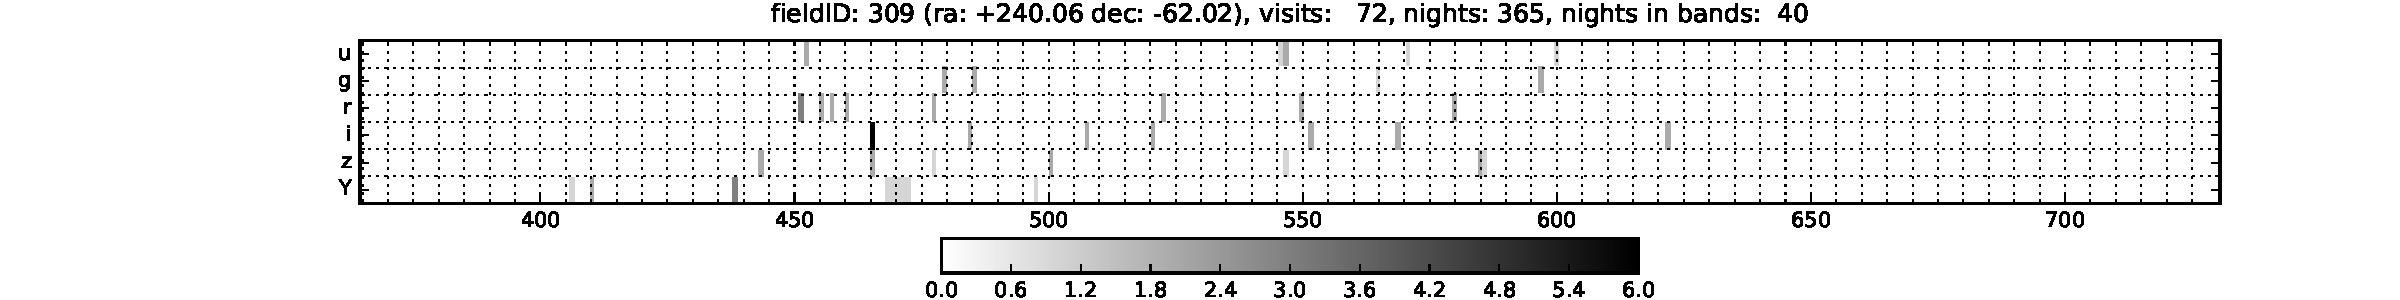
\includegraphics[width=\textwidth]{figs/supernova/fig_309_2ndYear}
 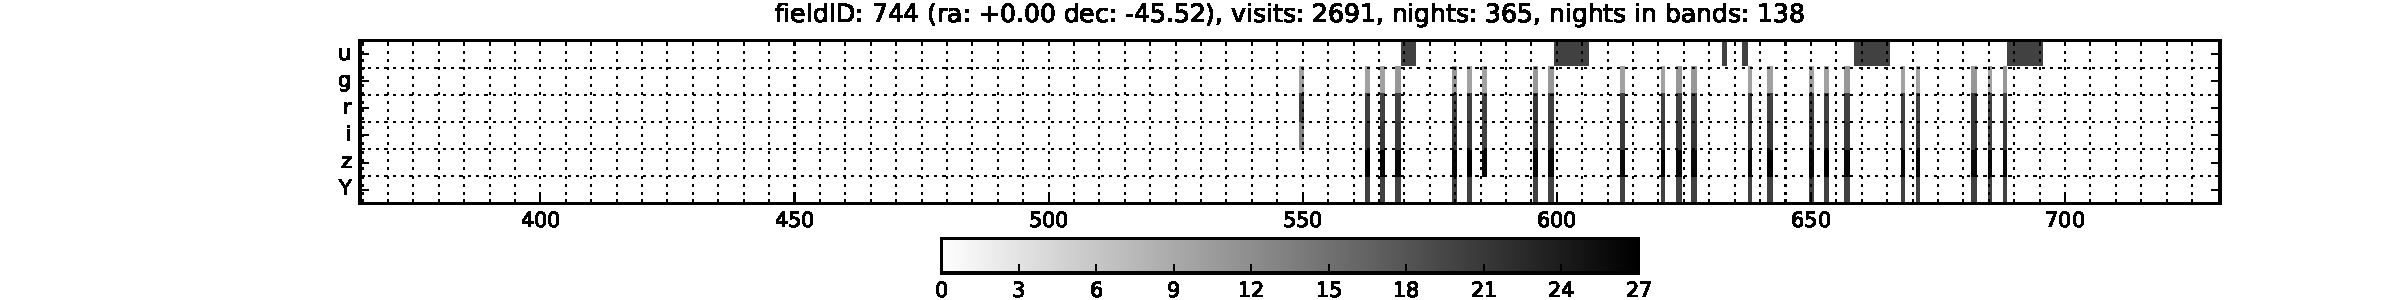
\includegraphics[width=\textwidth]{figs/supernova/fig_744_2ndYear}
 \includegraphics[height=0.2\textheight]{figs/supernova/loc_309_744.pdf}
 \caption{Example of the cadence in the 2nd season in a WFD Field
 (fieldID 309) (top-panel) and a Deep Drilling Field (fieldID 744)
 (middle panel) and the spatial location of these two fields shown on a
 map. The cadence plots show a heatmap of the number of observations per
 night during the second season in each filter u, g, r, i, z, y.
 The header shows the fieldID and location of
 the field, the total number of visits during that period, the number of
 distinct nights on which observations are taken, and the number of
 distinct observations (where observations are considered indistinct
 if they are on the same night and use the same band).}
  \label{fig:SN_sampling}
\end{figure}


\begin{figure}
\centering
 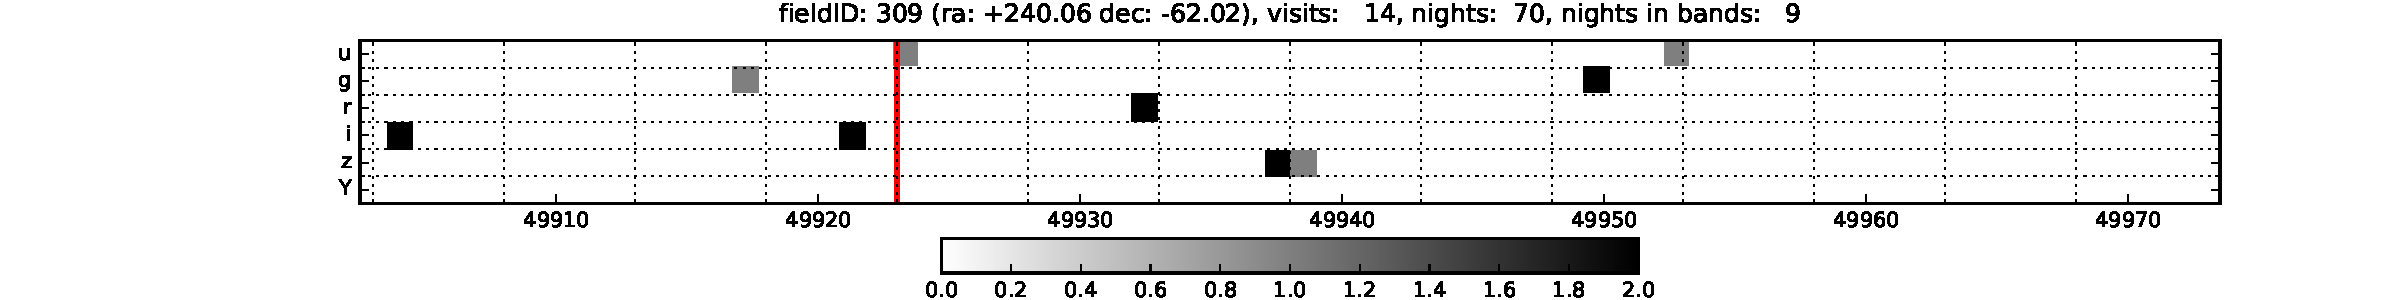
\includegraphics[width=\textwidth]{figs/supernova/TimeWindow_309_49923.pdf}
 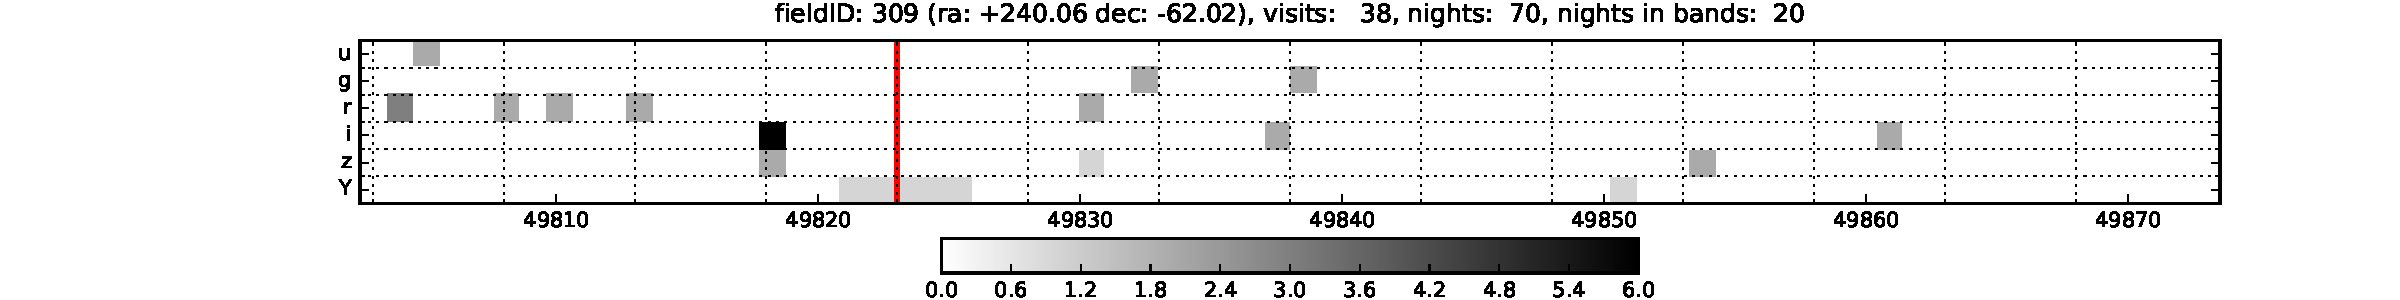
\includegraphics[width=\textwidth]{figs/supernova/TimeWindow_309_49823.pdf}
 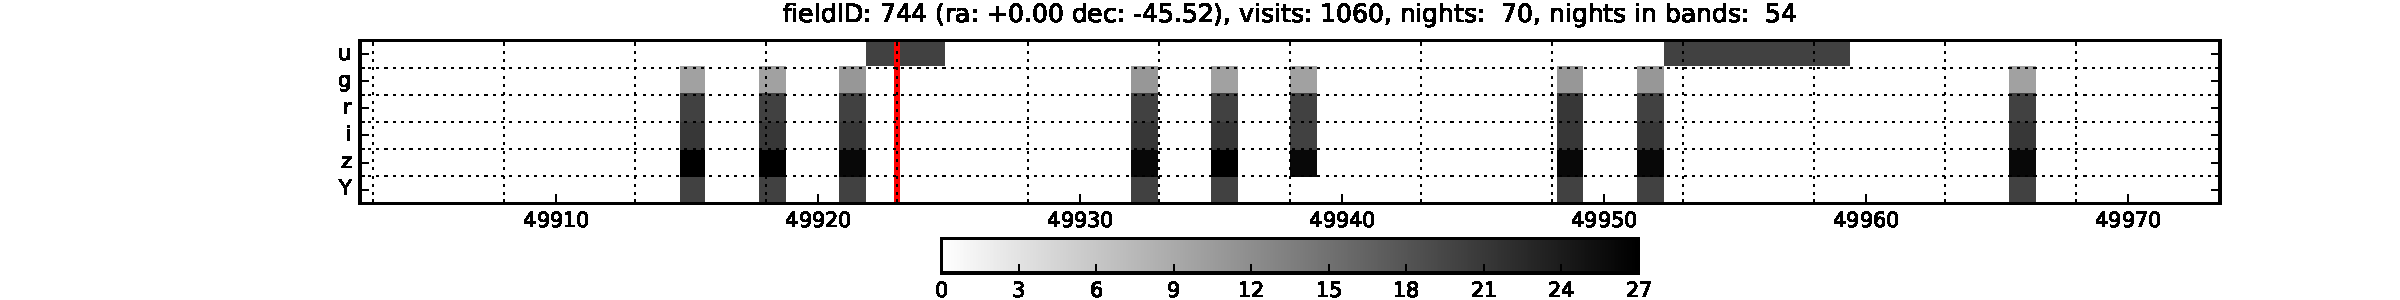
\includegraphics[width=\textwidth]{figs/supernova/TimeWindow_744_49923.pdf}
 %\includegraphics[height=0.2\textheight]{figs/supernova/loc_309_744.pdf}
 \caption{Example of a time window in a WFD Field (fieldID 309)
 (top-panel) and a second time window (middle panel) on the same field,
 and a Deep Drilling Field (fieldID 744) (bottom panel) all extending
 -20 days before and 50 days after a chosen night or MJD. For the Deep
 Drilling Field in the bottom panel, and the WFD field in the top
 panel, the chosen date around which the time window is constructed is
 the MJD of 49923, which is also 570 nights into the survey and marked
 by a red vertical line (which can be used to compare the location to
 \autoref{fig:SN_sampling}. The middle panel shows a window in Field
 309 centered around an MJD of 49823 or a night of 470 which may also be
 compared to \autoref{fig:SN_sampling}. The plots again show the
 heatmap of observations in each filter in each night as in the cadence
 plots of \autoref{fig:SN_sampling}.}
  \label{fig:TimeWindow}
\end{figure}

To define the metric $M,$ we need to define the perSNMetric. Two
different approaches to defining the perSNMetric for a given OpSim run are possible: a) Use
a simulated supernovae Type Ia with specific parameters, observed with
the sequence of observations in the above time window, and evaluate the
success of each step. b) Study heuristics of the observation sequences by using large simulations
with randomized parameter values. Here we will discuss the simpler approach (a).

%The SN metric in a spatial region
%reflects the contribution of the sample of SNe observed in that spatial
%region towards inferring the cosmological parameters. Let us
%consider a case where each SN observed with conditions better than a
%certain threshold contributes equally to the inference. Then the relevant
%metric would be a function of the number of SN in the sample passing
%such selection criteria. More generally, when the quality of all the
%supernovae are not similar, the metric should be thought of as
%the weighted sum of supernovae, with the weights being related to the
%inverse of the effective variance of the distance modulus:
%begin{equation}
%M\sim \sum_i w_i , \qquad  w_i \sim 1.0 /\sigma^2_\mu.
%\end{equation}
%By comparing with the form of the perSNMetric, we see that the
%perSNMetric should be a proxy for $1.0/\sigma^2_\mu,$ where
%$\sigma^2_\mu$ is the effective variance on the distance
%modulus of the supernova, as determined by fitting an empirical model to the supernova light curve.

%\subsubsection{ Steps in the PerSNMetric}
\subsubsection{Steps in the PerSNMetric}
\label{sec:persnmetric}
As described before, the measurement of the distance modulus is the
result of several steps. Therefore, we expect the perSNMetric to be a
product of metrics in each of the steps:

\begin{equation}
PM_i = \prod_{\rm{steps}} PM_i^{\rm{steps}}
\end{equation}

These components of perSNMetric constructed in different steps are
described in \autoref{tab:stepsAndMetrics}.
\begin{center}
 \begin{table}
\begin{tabular}{| p{5cm} |p{10cm}| }
\hline Metric & Description \\
\hline
I. SN discovery  (SNDM) &  Given the observations in a time window corresponding to the lifetime of
a supernova, evaluate the  probability of detecting a
transient. \\
II. SN classification (SNCM) & Given the observations in a time window corresponding to the
lifetime of a
supernova, evaluate the probability of accurately classifying the transient as a type Ia.\\
III. SN light curve characterization quality (SNQM) & Given the observations in a time window
corresponding to the lifetime of a supernova, evaluate the quality of characterization.\\
\hline
\end{tabular}
\caption{Components of the perSNMetric}
\label{tab:stepsAndMetrics}
\end{table}
\end{center}



\emph{I. Discovery Metric}

This metric is designed to gauge the performance of detection of SNe
discussed in \autoref{sec:\secname:targets}.
This metric is a proxy for the potential for a supernova to be detected
 during its lifetime by the set of images taken in different bands by LSST. The actual
 detection of SN during LSST is likely to use more stringent criteria, leading to 
 smaller numbers of supernovae in order to deal with possibly large numbers of false positives in detection. A larger
 number of images taken at a time when the supernova is bright enough increases the
 probability of detection. Technically, assuming that a single detection in any of the images containing
 the supernova is sufficient to trigger photometry at the location, one can find the
 probability of detection from an SNR vs. efficiency of detection curve. The signal-to-noise ratio
(SNR) can be determined given properties of a supernova (redshift, intrinsic brightness etc.)
 and the five sigma depth provided in OpSim. While such a SNR-efficiency curve does not
 yet exist for the LSST pipeline, one can use such a curve from previous surveys, in particular a
 SNR-efficiency curve constructed during a stage of the Dark Energy Survey for g, r, i, z bands of DES
 \citep{Kessler2015}. This is shown in \autoref{fig:SNR_detection}.
\begin{figure}
 \centering
 \includegraphics[width=\textwidth]{figs/supernova/SNR_detection.pdf}
 \caption{Probability of detecting a transient from a single difference image in different bands as
a
 function of the signal-to-noise as obtained from Dark Energy Survey \citep{Kessler2015}. It shows,
that
for high SNR greater than $\sim 10,$ a single exposure used in difference imaging may be sufficient to detect the SN, while for
lower SNR, several such image differences may be necessary to have a high probability of
detection.}
 \label{fig:SNR_detection}
\end{figure}

Using this information, one can compute the probability that a SN with given properties
will be discovered if from a set of images where the SN have a known signal to noise ratio. We use this as the
value for the supernova discovery metric (SNDM). While very high redshift (and thus faint)
supernovae will not be discovered, it is
potentially possible to discover many supernovae whose light curves will in turn not be well
characterized or hard to classify.


\emph{II. Classification Metric}

Separating supernovae from other detected transients is being considered in
\autoref{chp:transients}. Here we concern ourselves with problem of classifying subclasses of
SNe. Multiple techniques have been proposed to solve this problem \citep{Frieman2008,sako2008, kessler2010b, 
ishida2012, sako2014} and it is not yet clear how the
relative success of these techniques are affected by observing strategy. Work is ongoing to use the
multifaceted, machine learning pipeline developed in \citet{Lochner2016} to compare alternative
observing strategies. As this pipeline employs a variety of different feature extraction and machine learning
techniques, it is ideal to investigate the effect of observing strategy on the supernova classification. The exact 
metric used to determine the efficacy of the classification depends
on the exact problem at hand. For producing a general purpose, well-classified set of all types of
supernovae (for example, to study supernova population statistics), one could use the AUC metric
used in \citet{Lochner2016}, which is a good balance between purity and completeness. Ideally,
one would like a metric to be evaluated per object and included in the PerSNMetric. This is,
however, challenging as the success of classification will depend strongly on the nature of the
available training set, which will in turn depend on the spectroscopic follow-up program of LSST
and the availability of additional training data. Once a training set is determined and the
classification algorithm trained, a useful per-object metric is the classification probability of an
object being a Ia, which will be higher if the light curve is well-measured. This probability is
confounded by other factors (for example, other types appearing similar to Ia's), making
classification a very difficult metric to include on the per-object level. This is therefore left for future work.


\emph{III. Quality Metric}

We construct the quality metric for the perSNMetric by obtaining the
light curve of the SN in the time window described above. We fit the
light curve, using the SALT2 model \citep{Guy2007,2014A&A...568A..22B}, and approximately estimate the uncertainty in
distance from
the light curve fit alone. Of course, as is well known, luminosity
distance estimates of supernova Type Ia also show an intrinsic scatter
of around $0.1$ in previous surveys, which may be expected to decrease
with better training samples and understanding of underlying
correlations of SN Ia properties and their environments. We compute a
quality metric for each SN Ia as the ratio of the square of the
intrinsic dispersion to variance of the distance indicator from the supernova. 
$$ QM = 0.05^2/\sigma^2_{\mu}.$$ If our sample had a perfect discovery rate, and good classification (for example if we had spectroscopic classification), the uncertainty on
cosmological parameters would be entirely due to this quality metric and would be expected to scale with the quality metric as 
$$\frac{1}{\sigma} \sim \sqrt{\sum{\frac{1.0}{1.0 + 1.0 / QM}}}$$
where the sum is over the SNe in the sample.

%Move this to OpSim analysis
% The quality metric evaluated on the example SN plotted is $1.0$ if observed in the deep field
% (\autoref{fig:SNIaLCopsimdeep}), and $0.002$ in the WFD field (\autoref{fig:SNIaLCopsimmain}).



% --------------------------------------------------------------------

\subsection{OpSim Analysis}
\label{sec:\secname:analysis}
The scientific goal of characterizing SNe is, to a large extent, dependent
on how well the light curves of individual SNe are sampled in time and
filters. To study this, we re-index the OpSim output on spatial
locations rather than use the temporal index. Here, we first illustrate
in terms the cadence in two example LSST fields.

% {\bf Analysis, Results and Discussion}


% \begin{figure}[tbh!]
% %\vskip -1.3in
% \includegraphics[angle=0,width=0.99\hsize:,clip]{figs/SN_309_lcavg.pdf}
% %\vskip -1.3in
% \caption{Time-interval averaged light curve of
% \autoref{fig:SNIaLCopsimmain}. The light curve shows only a small number
% of the data points, which is insufficient to classify this object as a
% Type Ia and may be also difficult to classify this object as a SN. }
% \label{fig:SNIaLCopsimmain2}
% \end{figure}







% \begin{figure*}[!hb]
%     \begin{minipage}[b]{\linewidth}
%         \includegraphics[width=\textwidth]{figs/supernova/fig_firstSeason_0}
%         \includegraphics[width=\textwidth]{figs/supernova/fig_firstSeason_1}
%         \includegraphics[width=\textwidth]{figs/supernova/fig_firstSeason_2}
%         \includegraphics[width=\textwidth]{figs/supernova/fig_firstSeason_3}
%         \includegraphics[width=\textwidth]{figs/supernova/fig_firstSeason_4}
%     \end{minipage}
% \label{fig:opsimSummary}
% \caption{Cadence of Observations in the timewindow of a year towards a few sample of
% positions. Grey-scale indicates the number of visits. {\it add details}
% }
% \end{figure*}


We analyzed the OpSim output of the Baseline Observing Strategy,
enigma$\_$1189$\_$sqlite.db{\footnote
{\url{http://ops2.tuc.noao.edu/runs/}}} which includes Deep Drilling
Fields (DDF) and the main survey (WFD). While this is no longer the current baseline observing
strategy, we do not anticipate our conclusions would change with the use of
\texttt{minion\_1016}. Future work will include repeating our analyses with new OpSim runs, such as
\texttt{kraken\_1043}, which does not enforce visit pairs, and the new experimental rolling
cadences.

Using the OpSim output \texttt{enigma\_1189}, we generated
light curves for a type Ia supernova with a redshift of z=0.5 at a few different
locations. A date in MJD is chosen where the LSST simulated data are
reasonably well populated. We used the SALT2-extended model
with $x_0$, $x_1$ and $c$ set so that the SN Ia would have a specific
magnitude of $-19.3$ in the rest frame BessellB band. This was performed
using a version of \texttt{SNCosmo} to interpolate the SALT2 surfaces, and the
LSST catalog simulation package to calculate the flux for LSST
bandpasses.


\autoref{fig:SNIaLCopsimdeep} shows the light curve in
different filters in a deep drilling field. The
number of visits for 50 days (which is the period of the simulated SN Ia light curve in
rest-frame, which translates to 75 days at z=0.5) is 53 per filter. For this light
curve, the supernova quality metric (SNQM) and the
discovery metric (SNDM), are both equal to 1. SNDM=1 indicates that this object is a transient that
will be definitely discovered, and SNQM=1 indicates that the light
curves will be of high quality enough to contribute extremely well to
the inference of cosmological parameters. The light curves and
quantified metric demonstrate that data from Deep Drilling Fields would
generate high quality light curves, allowing a high rate of supernova
discovery.

In contrast, \autoref{fig:SNIaLCopsimmain} shows a light curve from the WFD survey. This light
curve is
generated in Field 290 and has an average number
of data points in the light curve of 2 per filter. Using these light
curves, the probability (SNDM) of detecting this supernova is less
than 0.1. \autoref{fig:perSNCadence} directly compares the light curves and cadences of the two
fields considered, from the DDF and WFD.

\begin{figure}
%\vskip -1.3in
%*\includegraphics[angle=0,width=0.99\hsize:,clip]{figs/SN_290_lc.pdf}
\centering
\includegraphics[angle=0,width=14truecm]{figs/supernova/SN_290_lc.pdf}
%\vskip -1.3in
\caption{An example of a light curve, in six filter bands, of a SN Ia from the DDF field with fieldID 290 in
\texttt{enigma\_1189}.
}
\label{fig:SNIaLCopsimdeep}
\end{figure}

\begin{figure}
%\vskip -1.3in
\centering
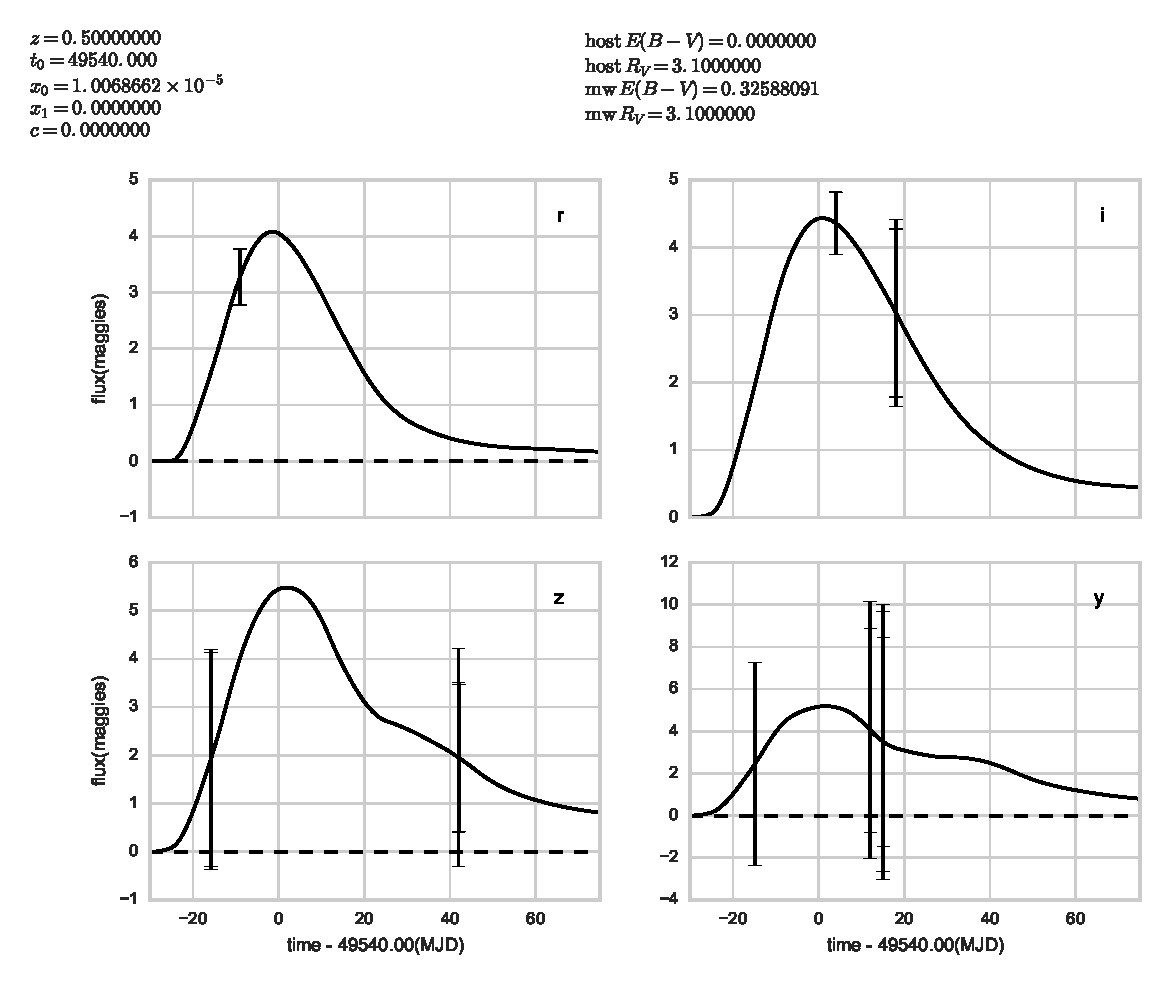
\includegraphics[angle=0,width=0.99\hsize:,clip]{figs/supernova/SN_309_lc.pdf}
%\vskip -1.3in
\caption{An example of a light curve, where only four filter bands are available, of a SN Ia from
the WFD survey in
\texttt{enigma\_1189}.
}
\label{fig:SNIaLCopsimmain}
\end{figure}

\begin{figure}
\centering
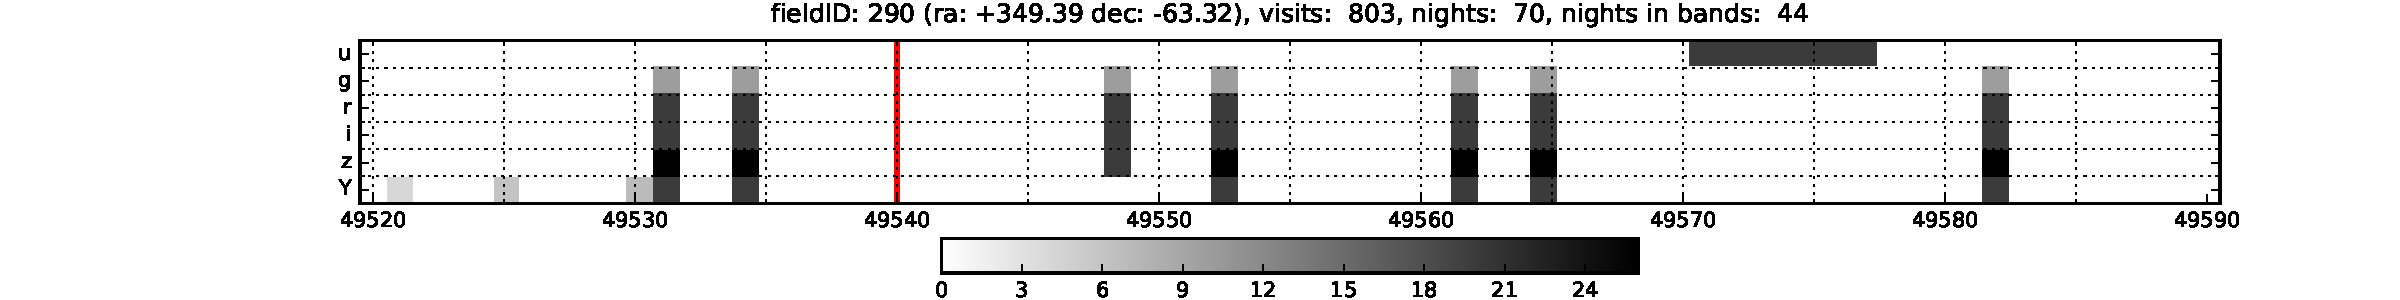
\includegraphics[angle=0,width=\textwidth,clip]{figs/supernova/SN_Cadence_290.pdf}
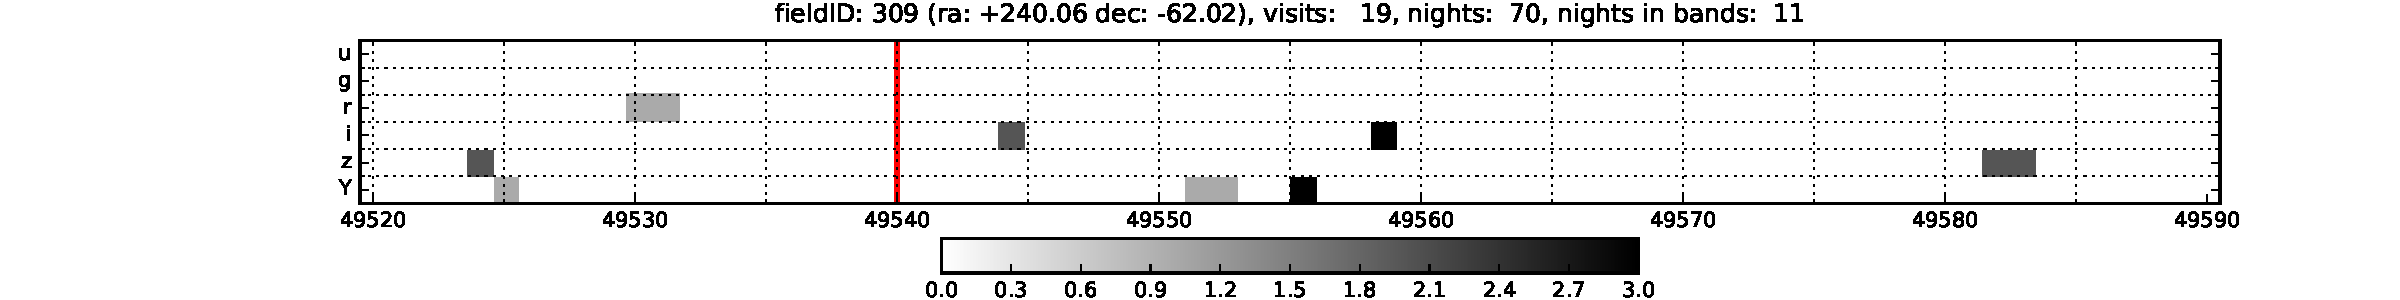
\includegraphics[angle=0,width=\textwidth,clip]{figs/supernova/SN_Cadence_309.pdf}
\caption{Cadence of observations in the time window of a representative
supernova at redshift of $z=0.5$ in a DDF (top) field (fieldID: 290) and
a WFD (bottom) field (fieldID: 309). The red lines show the date of
peak, and the shades show the number of observations in a night in
a distinct filter.}
\label{fig:perSNCadence}
\end{figure}

{\bf Analysis Results:}
To further study the quality of light curves across the survey, we simulate the same type Ia
supernova in 16 different fields, including DDF 290 already studied, from the \texttt{enigma\_1189}
OpSim run and record the average number of visits per 50 day time window
(\autoref{tab:lcpositions}). A well-known rule of thumb (R. Foley, priv. communication) for good
quality SN light curves is to
demand 7-10 epochs per light curve spread over 50 days or so for more than one filter.
\autoref{tab:lcpositions} list characteristics of light curves towards 15 fields in the OpSim
output.

We summarize results of light curve analysis using OpSim output as follows:
\begin{itemize}
\item A high portion of the light curves, in both the WFD and DDF, can be identified as transients
using  the SN
discovery metric (SNDM$>$0.5 in \autoref{tab:lcpositions}).
This metric is currently using SNR of detections.
\item Light curves from WFD show poor qualities (SNQM$<$0.3) whereas the light curves from DDF show
high quality ($\geq$1). Note that we examined only a few cases of SNe at redshift of 0.5 and the
metric will be applied to a much larger range of SNe in future simulations.
\item We have explored ways to improve SN classification \citep{Lochner2016} and the classification
metric is described in Section
\ref{sec:\secname:metrics}.
In this analysis, we have not yet considered classification based on individual light curves.
This is because, unlike the discovery and quality metric, it is difficult to discuss
classification of a single object without having a well-defined training set, which is yet to be
determined for LSST.
\item In conclusion, based on the SNQM, we have showed that WFD data alone using the Baseline
Observing Strategy are not useful for SN studies.
\end{itemize}


%Although
%the averages in \autoref{tab:lcpositions} are only approximations because the cadence is
%non-uniform, they give a clear indication that with the \texttt{enigma\_1189} observing strategy,
%the WFD will not be useful for SNe studies.

{\bf Need for LSST observing strategy optimization for SN science:}

The results from our OpSim analysis motivate our proposal of a rolling cadence
in order to improve the sampling of SNe over a much larger area than the DDFs.
The DDF are useful for SNe at redshifts between 0.6 and 1.2, and the WFD will help us to increase
the number of SNe at low redshift
as shown in Figure 11.1 of LSST science book \citep{2009arXiv0912.0201L}. For example, a higher
number of SNe at z $=0.4$ is expected from WFD than DDF.
Consequently, DDF will have only a few SNe at low redshift,
since the DDF sample is limited to small patches of sky.
A significant scatter in distance modulus of low redshift SNe is found \citep[e.g.][]{Suzuki2012} which hinders deriving accurate
cosmological parameters.
Since the cosmology measurement requires low as well as high redshift distance moduli, a large
sample
of low redshift SNe will improve the cosmological parameter inference. The WFD would also provide a
useful sample of nearby supernovae to better constrain variations in SNe populations (for both
type Ia and core-collapse SNe).
Light curves from WFD
with reasonable quality can be achieved using our new proposed
observing strategy.

A larger sample of well-characterized light curves from the WFD can address two key science
goals:
\begin{itemize}
\item Tightly constraining cosmological parameters ($\Omega_M$ and $\Omega_\Lambda$)
by improving the measurement of distance modulus of low redshifted SNe. Without implementing
the new observing strategy that we recommend below, LSST will not be able to
make a significant contribution to SN cosmology below z$<$0.5.
\item The WFD offers a unique opportunity for isotropy studies (complementary to large-scale galaxy
surveys) and dynamical dark energy studies. Apparent luminosities and number counts can be
estimated for a large range of angular scales and
redshifts with WFD. However, this science case will only be possible with a large sample of
well-characterized SN Ia in a large field of view, providing further support for our
recommendation of a rolling cadence observing strategy.
\end{itemize}



% [ML] I've removed this (fairly arbitrary) chategorization, it's more confusing than helpful
% and it's clear how bad WFD is from the numbers alone

% In column 5, we categorize the positions into 5 categories
% base on the data points (the value in column 3) per filter for 50 days.
% When the number of LSST data points (the value in column 3) per filter
% for 50 days is $>$9 as the category A, 5-9 as B, 1.8 -- 5 for C, 1 --
% 1.8 for D, and $<$1 for E. An example of light curve of Category A has
% been shown in Figure \ref{fig:SNIaLCopsimdeep}, Examples light curves of
% Category B have been shown in Figures \ref{fig:SNIaLCopsimmain} and
% \ref{fig:SNIaLCopsimmain2}, respectively. An example of a light curve of
% Category C (ex. Dec.=-40 ;No. 7 in Table \ref{tab:lcpositions}) is shown
% in \autoref{fig:SNIaLCminus40}.

% \new{An example of Category B toward -66$^{\circ}$ is shown
% \autoref{fig:SNIaLCminus66} (No. 3 in \autoref{tab:lcpositions}). The
% light curves in {\it u, g} and {\it r} bands have 3 -- 5 data points,
% while {\it i} band has 8 or more than data points. The band z and y show
% relatively large error bars. In order to increase probability to
% recognize the light curve as a SN and Type Ia, simulated LSST data
% points could be increased by a factor of 2-3. Our goal is to improve the
% light curves which belong to Category B and C so that we can distinguish
% them as a SN and particularly as a Type Ia SN. This will improve values
% in SNDM and SNQM.}

\begin{center}
\begin{table}
%\tabletypesize{\scriptsize}
\centering
\begin{tabular}{|p{1.3cm} |p{3.3cm}|p{4cm}|p{1.9cm}|p{1.7cm}|p{1.7cm}|}
%\begin{tabular}{|p{0.9cm} |p{3.3cm}|p{4cm}|p{1.9cm}|}
\hline
 FieldID & (R.A., Decl.) & Number of LSST visits per year (u,g,r,i,z,y)       & Number of Avg. data
per SN period per filter & SNDM  & SNQM\\
\hline
290 DDF  & (349.386,-63.321)  & 2363 (398,229,402,414, 522,396) & 53 & 1.0  & 1.6 \\
 17      & (190,-83) &    239 (38,41,41,44,33,42) & 5.3 & .. & ..\\
% 290  &(20,-83) & 252 (52,56,40,21,37,44)  &5.7 &&\\
 22      &(20,-83) & 252 (52,56,40,21,37,44)  &5.7 &..&..\\
%old 3      &(120.012,-71.879) &  220(36,38,37,32,44,33) & 5.0 & B &\\
  217      &(116,-66) &  220 (36,38,37,32,44,33) & 5.0  & .. & ..\\
% 290(+DDF)  &(116,-66) &  220 (36,38,37,32,44,33) & 5.0  && 1.0 & 8.28\\
 309      &(240.05,-62.02) &101 (2,5,11,19,19,45) & 2.2 & 1.00 & 0.10  \\
 645      &(120,-50)  &80 (4,7,9,18,24,18)        & 1.8 &0.54 & 0.01\\
 949      & (80,-40)  &      96 (5,8,15,17,27,24) &  2.2 & 0.99 & 0.09\\
 948      & (280,-40) &      86 (4,2,6,4,24,18)   &  2.0 & 0.99 & $<$0.002\\
 1401      & (58,-27)   & 98 (3,3,9,26,31,26) &   2.2 & 0.77 & 0.002\\
 1754      & (30,-20)  &      86 (3,4,10,21,27,21) &  2.0 & 1.00 & 0.05\\
 1720      & (100,-20) &      58 (4,2,6,4,24,18)   &  1.3 & 0.99 & 0.03 \\
% 000  & (358.41,+0.18)  &                      &     & C({\it 0.1}) & \ref{fig:SNIaLCDecp18}\\
 2556  & (6.097, -1.105) & 80 (4,7,9,18,24,18)  & 1.8 & 1.00 & 0.05\\
% 290  & (6.097, -1.105) &                      &     & C({\it 0.1}) & \ref{fig:SNIaLCDecp18}\\
 2718     & (50,+1.5) &      72 (3,6,10,12,22,19) &  1.6 & 1.00 & 0.09\\
 2751     & (320, +5) &      7 (0,0,2,0,4,0)      &  0.2 & 0.09 & 0.02\\
% 2910     & (60,+5)   &      66 (0,7,11,20,28,0)  &  1.5 &.. & ..&\\
 3606     & (60,+20)  &      72 (0,8,13,22,29,0)  &  1.6 &..& ..\\
% 3959     & (60,+30)  &      44 (0,5,6,15,18,0)   &  1.0 &&\\
\hline
\end{tabular}
\caption{Table of 15 fields in the OpSim run \texttt{enigma\_1189}. The first column is simply an
index, with the special example fields of the DDF field 290 indicated. The
position of the fields is shown in column 2. The third column contains the total and per filter
band number of visits per year and this is averaged per filter per 50 day time window in column 4.
It can be seen that with this observing strategy, only the deep drilling fields are suitable for
supernova cosmology, where 7-9 data points per filter band is considered adequate quality. SNDM and
SNQM are SN discovery and quality metric, respectively, in the last two columns. Note that the
metric measurements are missing for some entries due to a spatial mismatch in fields that will be
rectified in future.}
\label{tab:lcpositions}
\end{table}
\end{center}

% \begin{center}
% \begin{table}
% %\tabletypesize{\scriptsize}
% \begin{tabular}{|p{0.7cm} |p{2.8cm}|p{4cm}|p{1.7cm}|p{1.4cm}|p{0.7cm}|}
% \hline
%  Field or No. & (RA,Dec) & No. of LSST data per year (u,g,r,i,z,y)       & Avg. No.&Category (TPR)
% &Fig. No. \\
% % Field or [No.] & (RA,Dec) & No. of LSST data per year (u,g,r,i,z,y)       & Avg. No. per filter
% per 50 days   &Category (TPR)\\
% %  or No.      &  (J2000)  & per year (u,g,r,i,z,y) & per filter & (TPR)    \\
% %        &           &                        & per 50days &     \\
% 290 DDF  & (349.386,-63.321)  & 2363(398,229,402,414, 522,396) & 53 &
% A(1)&\ref{fig:SNIaLCopsimdeep}
%  \\
%  1      & (190,-83) &    239(38,41,41,44,33,42) & 5.3 & B ({\it 0.4}) & \\
%  2      &(20,-83) & 252(52,56,40,21,37,44)  &5.7  & B  & \\
% %old 3      &(120.012,-71.879) &  220(36,38,37,32,44,33) & 5.0 & B &\\
% 3      &(116,-66) &  {\it 220(36,38,37,32,44,33)} & 5.0 & B & \ref{fig:SNIaLCminus66} \\
%  4      &(240.05,-62.02) &101(2,5,11,19,19,45) & 2.2  & B & \ref{fig:SNIaLCopsimmain2}\\
%  5      &(120,-50)  &80(4,7,9,18,24,18)        & 1.8 &  C &\\
%  6      & (80,-40)  &      96(5,8,15,17,27,24) &  2.2 & C &\\
%  7      & (280,-40) &      86(4,2,6,4,24,18)   &  2.0& C &\\
%  8      & (30,-20)  &      86(3,4,10,21,27,21) &  1.96& C & \\
%  9      & (100,-20) &      58(4,2,6,4,24,18)   &  1.3& D &\\
% % 000  & (358.41,+0.18)  &                      &     & C({\it 0.1}) & \ref{fig:SNIaLCDecp18}\\
%  309  & (6.097, -1.105) & 80 (4,7,9,18,24,18)  & 1.83   & C({\it 0.1}) & \ref{fig:SNIaLCDecp18}\\
% % 290  & (6.097, -1.105) &                      &     & C({\it 0.1}) & \ref{fig:SNIaLCDecp18}\\
%  11     & (50,+1.5) &      72(3,6,10,12,22,19) &  1.64& D &\\
%  12     & (320, +5) &      7(0,0,2,0,4,0)      &  0.15& E &\\
%  13     & (60,+5)   &      66(0,7,11,20,28,0)  &  1.5  & D& \\
%  14     & (60,+20)  &      72(0,8,13,22,29,0)  &  1.64& D &\\
%  15     & (60,+30)  &      44(0,5,6,15,18,0)   &  1.0& E &\\
% \hline
% \end{tabular}
% \label{tab:lcpositions}
% \end{table}
% \end{center}


% \emph{To be added: 2 more examples of light curves at different positions of sky.}

% \begin{figure}[tbh!]
% %\vskip -1.3in
% \includegraphics[angle=0,width=0.99\hsize:,clip]{figs/supernova/LCDecminus40no40.pdf}
% %\vskip -1.3in
% \caption{An example of light curve of SN Type Ia (Dec. of -40$^{\circ}$: No. 6) using
% the Main Survey of the LSST Baseline OpSim run. }
% \label{fig:SNIaLCminus40}
% \end{figure}
%
% \begin{figure}[tbh!]
% %\vskip -1.3in
% \includegraphics[angle=0,width=0.99\hsize:,clip]{figs/supernova/s1_lc_coaddedDecminus66RA115.pdf}
% %\vskip -1.3in
% \caption{An example of light curve of Type Ia in the direction to Dec. of -66$^{\circ}$
%  using the Main Survey of the LSST Baseline OpSim run.
% }
% \label{fig:SNIaLCminus66}
% \end{figure}
%
%
% \begin{figure}[tbh!]
% %\vskip -1.3in
% \includegraphics[angle=0,width=0.99\hsize:,clip]{figs/supernova/LCfield00Decp18RA358.pdf}
% %\vskip -1.3i
% \caption{}
% %\caption{An example of light curve of Type Ia in the direction (RA, Dec.)=(358.41, +0.18)
% % using the Main Survey of the LSST Baseline OpSim run. A representative lightcurve
% % of Category C.
% %}
% \label{fig:SNIaLCDecp18}
% \end{figure}

% --------------------------------------------------------------------
%
% \subsection{Conclusions}
%
% Here we answer the ten questions posed in
% \autoref{sec:intro:evaluation:caseConclusions}:
%
% \begin{description}
%
% \item[Q1:] {\it Does the science case place any constraints on the
% tradeoff between the sky coverage and coadded depth? For example, should
% the sky coverage be maximized (to $\sim$30,000 deg$^2$, as e.g., in
% Pan-STARRS) or the number of detected galaxies (the current baseline 
% of 18,000 deg$^2$)?}
%
% \item[A1:] ...
%
% \item[Q2:] {\it Does the science case place any constraints on the
% tradeoff between uniformity of sampling and frequency of  sampling? For
% example, a rolling cadence can provide enhanced sample rates over a part
% of the survey or the entire survey for a designated time at the cost of
% reduced sample rate the rest of the time (while maintaining the nominal
% total visit counts).}
%
% \item[A2:] ...
%
% \item[Q3:] {\it Does the science case place any constraints on the
% tradeoff between the single-visit depth and the number of visits
% (especially in the $u$-band where longer exposures would minimize the
% impact of the readout noise)?}
%
% \item[A3:] ...
%
% \item[Q4:] {\it Does the science case place any constraints on the
% Galactic plane coverage (spatial coverage, temporal sampling, visits per
% band)?}
%
% \item[A4:] ...
%
% \item[Q5:] {\it Does the science case place any constraints on the
% fraction of observing time allocated to each band?}
%
% \item[A5:] ...
%
% \item[Q6:] {\it Does the science case place any constraints on the
% cadence for deep drilling fields?}
%
% \item[A6:] ...
%
% \item[Q7:] {\it Assuming two visits per night, would the science case
% benefit if they are obtained in the same band or not?}
%
% \item[A7:] ...
%
% \item[Q8:] {\it Will the case science benefit from a special cadence
% prescription during commissioning or early in the survey, such as:
% acquiring a full 10-year count of visits for a small area (either in all
% the bands or in a  selected set); a greatly enhanced cadence for a small
% area?}
%
% \item[A8:] ...
%
% \item[Q9:] {\it Does the science case place any constraints on the
% sampling of observing conditions (e.g., seeing, dark sky, airmass),
% possibly as a function of band, etc.?}
%
% \item[A9:] ...
%
% \item[Q10:] {\it Does the case have science drivers that would require
% real-time exposure time optimization to obtain nearly constant
% single-visit limiting depth?}
%
% \item[A10:] ...
%
% \end{description}

% --------------------------------------------------------------------

\subsection{Discussion}
For \texttt{enigma\_1189} (and also, most likely, for the current baseline strategy), the DDF
fields will produce an exquisite sample of
well-characterized SNe for cosmology and astrophysics studies. Further analysis is required to
determine exactly how many (useful) supernovae will be detected and what the resulting cosmological
constraints will be, but in this section we have discussed and motivated several important
intermediate metrics.

\subsubsection{Scientific motivation for rolling cadence}
It is clear from the above analysis, that the WFD component of the LSST survey will not be useful
for supernova cosmology. However, with some changes to the observing strategy, it is likely that a
large part of the WFD can be leveraged by implementing a rolling cadence strategy. The idea is to
sample a particular field with much higher cadence, at the expense of other fields, for a period of
time (such as 50-100 days) and change fields throughout the survey to preserve uniformity by the end
of the 10 year period.
%Ideally, we would propose changing the filter every day, and trebling the
%average WFD cadence in these smaller fields.
Our aim is to achieve 7-9 points per light
curve over a 50 day period, which would produce light curves of reasonably high quality, that
can be well-classified and well-characterized for cosmological parameter estimation.

\subsubsection{Proposed observing strategy optimized for SN cosmology}

We propose a new observing strategy that provides a dense sampling in time, to improve the
observing strategy of the WFD survey in order to produce SN light curves which are
more useful for SN studies.
We suggest to increase the sampling rate by a factor of 2 or more, and we choose the best option for the sampling rate
to be enhanced by a factor of 3 ($\times$3 hereafter).
%We use an increase of the sampling rate by a factor of 3 for our proposed Cadence, hereafter.
An example of light curve generated with current Universal cadence
and with $\times$3
enhanced light curve is shown in Fig. \ref{fig:LCrandom}.
The enhanced light curve is generated by drawing randomly from a uniform distribution over the
length of the light curve and predicting the flux from the underlying Ia model.

\begin{figure}
\centering
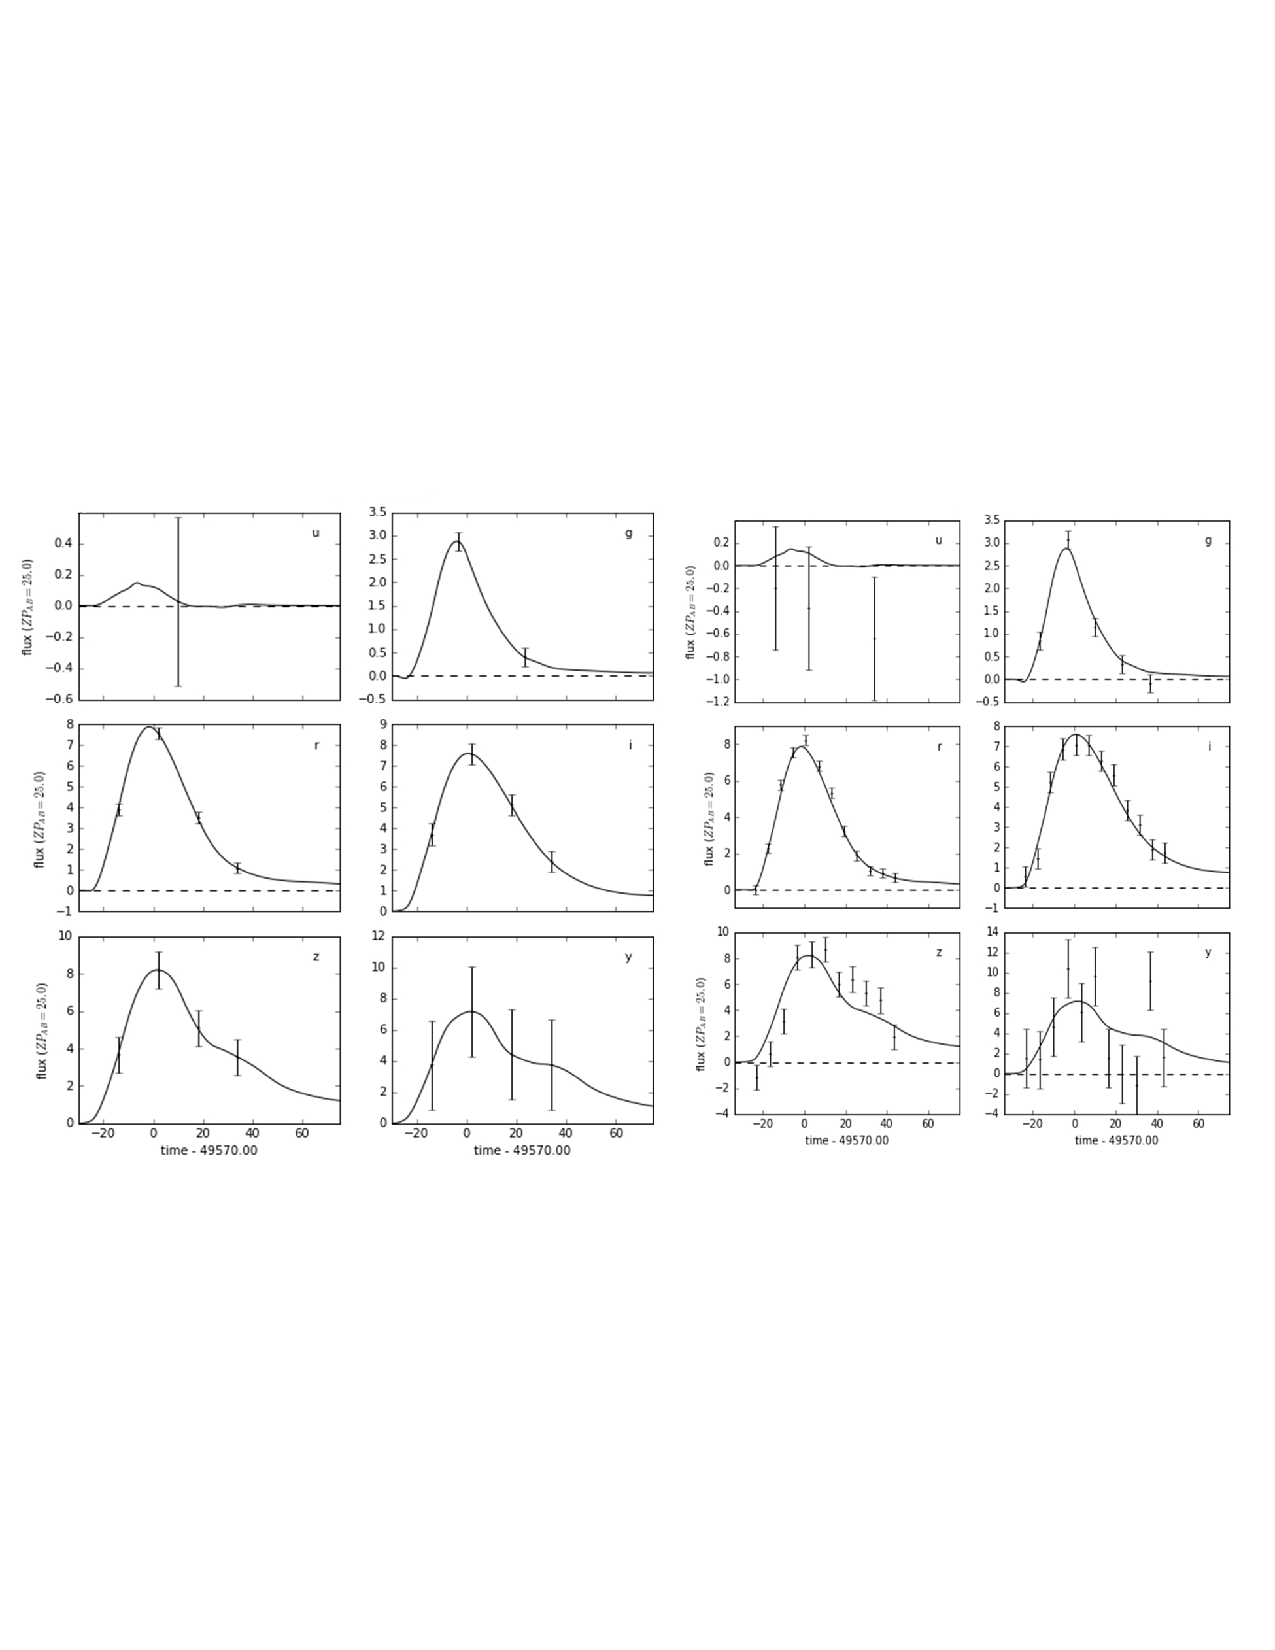
\includegraphics[width=13truecm]{figs/supernova/LCrandomseed.pdf}
\caption{An example of light curve of SN Type Ia generated using OpSim output
at RA. of 58$^{\circ}$ and Decl. of -27$^{\circ}$ (left) and the same light curve
after the sampling rate is enhanced by a factor of 3 (right).}
  \label{fig:LCrandom}
\end{figure}

\subsubsection{Details of rolling cadence of WFD optimized for SN cosmology }
%Ideally, we would propose changing the filter every day, and trebling the
%average WFD cadence in these smaller fields. Our primary goal is to  achieve our goal of 7-9 points per light
There are likely many possible LSST observing strategies one could propose to achieve our
goal of increasing the sampling of light curves by a factor of three. We hope to investigate
multiple OpSim runs in the future with a variety of implementations of rolling cadence.
In this section, we show a plausible observing strategy
that can achieve a factor of 3 increase in sampling rate in order to obtain reasonable-quality SN light curves.


The observing strategy of WDF is defined (see Section 1.6.2 in the LSST science book) as follows.

\noindent $\bullet$ A revisit time of three days on average per 10,000 deg$^2$ of sky (i.e., the area visible at any given time of the year), with two visits per night (particularly useful for establishing proper motion vectors for fast moving asteroids).

We define the 10,000 deg$^2$ survey area (the visible sky for a given time of the
year) simply as the ``visible sky".
In order to increase the sampling rate by a factor of 3, we propose to make the revisit time of $\sim$1 day (1/3 of three days above)
on average visible
sky. This means one third of the visible sky ($\sim$3300 deg$^2$) can be chosen. Preference
may be given to the part of
sky with low air-mass, but at the same time
a uniform coverage of LSST needs to be considered.
Ideally we would propose a filter change every day, and observe approximately the same
patch of visible sky for
$\sim$ 50 days before
going to another part.
As a result,
 the light curves will have  a sampling rate ($\times$3) in time.
A total of 1.4$\times$10$^5$ SNe Ia (Section 11.2.2 in \citet{2009arXiv0912.0201L}) expected from
WDF would become a factor of 2-3 lower
(details are to be investigated in future), but
the SNe that LSST WFD discovered will have  meaningful, reasonable-quality light curves which can be used to
classify the types of SNe and to improve cosmological parameters.

\subsection{Conclusion}

Here we answer the ten questions posed in Sub-section 1.2.1:

\begin{description}
\item[Q1:] {\it Does the science case place any constraints on the
tradeoff between the sky coverage and coadded depth? For example, should
the sky coverage be maximized (to $\sim$30,000 deg$^2$, as e.g., in
Pan-STARRS) or the number of detected galaxies (the current baseline 
of 18,000 deg$^2$)?}

\item[A1:] For supernova observations, the most important aspect is cadence: we need a
good sampling of well-measured light curves of supernovae. If the sky
coverage can be increased without sacrificing the number of observations
per supernova (i.e., over one season), such as using a rolling cadence
strategy, this will greatly improve supernova science. Inasmuch as
requiring increased sky coverage could negatively affect cadence over one
season, our preference is not to increase to a larger sky coverage.

\item[Q2:] {\it Does the science case place any constraints on the
tradeoff between uniformity of sampling and frequency of  sampling? For
example, a rolling cadence can provide enhanced sample rates over a part
of the survey or the entire survey for a designated time at the cost of
reduced sample rate the rest of the time (while maintaining the nominal
total visit counts).}


\item[A2:] Frequency of sampling is much more important than uniformity over long time
scales for all forms of supernova science. For SN Ia cosmology, light-curve
sampling should be about three times as frequent as for the current
baseline WFD cadence. While further investigation is needed, a reasonable
length of a season with enhanced rates is around 120-150 days. A rolling
cadence will allow this improved sampling while still keeping the sky
coverage and co-added depth, by concentrating on different fields in
different seasons (see Section 9.5 for details).

\item[Q3:] {\it Does the science case place any constraints on the
tradeoff between the single-visit depth and the number of visits
(especially in the $u$-band where longer exposures would minimize the
impact of the readout noise)?}

\item[A3:] In general for supernova science, the number of visits is more important to
the single-visit depth, though we would not advocate any decrease in
single-visit exposure time (below 2x15 sec). The U band  is useful for the
low-z (wide-area) sample and and their calibration of the Hubble diagram.
It is not obvious if longer exposures are helpful at this time for
supernova science.

\item[Q4:] {\it Does the science case place any constraints on the
Galactic plane coverage (spatial coverage, temporal sampling, visits per
band)?}

\item[A4:] Our supernova science is extragalactic and will use high Galactic-latitude
fields almost exclusively (to minimize Milky Way extinction systematic
uncertainties). Survey time spent on Galactic fields takes away from survey
time for our science; we would optimize for less time in the Galactic
plane.

\item[Q5:] {\it Does the science case place any constraints on the
fraction of observing time allocated to each band?}


\item[A5:] For supernova science, we have no strong preference for any band and would
benefit from roughly uniform depth per band. While redder bands are more
useful for higher redshift supernovae, the bluer bands are helpful
especially for lower redshift objects. Visits in each band should be
uniformly spread in time. A higher number of visits to redder bands is
preferred for DDF.

\item[Q6:] {\it Does the science case place any constraints on the
cadence for deep drilling fields?}


\item[A6:] Our optimal cadence would for the DDFs would be nightly or every other
night; every three nights would be acceptable. Beyond this we run the risk
of large gaps more than $\sim$7 days, which would be detrimental to supernova
science. Ideally, the DDFs would be observed in all available filters,
though not all filters are needed every night (so for instance some filters
could be observed on night 1, the others on night 2, and repeat). The
single-night depth should be 1-2 mag deeper than a WFD field, but not much
more; any extra time is better spent on a different night.

We would like a suitable number of extragalactic DDFs in total so that at
least a few ($\sim$3 to 5) are being observed at any time in the survey: we
would limit an increase in the number of DDFs if it came at the expense of
our preferred high cadence. Each field should be observed for a $``$season" of
length at least $\sim$120-150 days, staggering the fields so new fields cycle in
as old ones cycle out. In addition, for DDFs, the u-band exposure time
could be increased to minimize readout noise.

\item[Q7:] {\it Assuming two visits per night, would the science case
benefit if they are obtained in the same band or not?}



\item[A7:]Supernova science benefits enormously from having color information,
particularly in discovery and early epochs to help classification. Two
visits in the same band will be less useful than visits in different bands.

\item[Q8:] {\it Will the case science benefit from a special cadence
prescription during commissioning or early in the survey, such as:
acquiring a full 10-year count of visits for a small area (either in all
the bands or in a  selected set); a greatly enhanced cadence for a small
area?}



\item[A8:] During commissioning, we would like as many DDFs as possible observed in
all filters (with few times the per-night exposure time) so that templates
can be created for each of the DD fields we consider. This will allow us to
find useful supernovae in these DDFs as soon as the survey starts, and
provide us with useful time to deal with any issues in the image
subtraction etc. before the survey begins.

Early in the survey, we must build templates for all fields (more broadly
than just the DDFs). Our favored method for doing this is to devote the
bulk of year 1 to covering the full sky area, with a rolling cadence survey
commencing thereafter. As above, the templates should be at least a few
times the exposure time of a single visit (so that the template noise does
not dominate the subtraction). This is particularly important in the first
3-5 weeks of the survey, to ensure that we get useful data from the rest of
the critical first year.

\item[Q9:] {\it Does the science case place any constraints on the
sampling of observing conditions (e.g., seeing, dark sky, airmass),
possibly as a function of band, etc.?}


\item[A9:] While supernova observations benefit from good seeing, it is not as strong
a requirement as it is for other science cases. Moreover we would like to limit
any image coaddition issues for very good seeing (under the assumption that
these remain): we can make good use of observing conditions with slightly
poorer seeing.


\item[Q10:] {\it Does the case have science drivers that would require
real-time exposure time optimization to obtain nearly constant
single-visit limiting depth?}

\item[A10:]A sufficiently long (or nominal), fixed exposure time should be adequate
for supernova science. No real-time optimization is necessary, and
single-visit science is not the limiting factor for SNe science.


\end{description}



% \subsection{Rolling Cadence of the Main Survey Optimized for Supernova Science}
%
% \subsubsection{ Scientific Motivation for Rolling-Cadence}
%
% The main survey is important for the discovery of supernovae (SNe) in
% the redshift range of 0.1- 1, which is critical to constraint SN
% cosmological parameters. In order to identify a variable source as a SN
% and to distinguish the source as a Type Ia SN, we need 7-10 epochs
% spread over 45 days or so for each filter based on past experience.
% Universal survey of the Baseline Cadence provides 6 filter data for
% approximately 18 days (assuming a survey with a filter can be done for 3
% days). This provides 15 data points over 45 days and 2.5 data points in
% average for each filter. Our analysis of OpSim run (Baseline Observing
% Strategy) output shows the light curves of SNe from the OpSim data are
% insufficient not only to identify the source as a SN and but also to
% classify the SN if the SN is type Ia or II (or Ib, Ic). Our proposed
% observing strategy is critical to improve the quality of SN light
% curves. The light curves will have at least 3 times densely populated
% data points in time.
%
%
% \subsubsection{Proposed Rolling-Cadence of the Main Survey Optimized for SN Science }
%\label{sec:\secname:discussion}

% {\it Discussion: what risks have been identified? What suggestions could be
% made to improve this science project's figure of merit, and mitigate
% the identified risks?}
%
% Our goal for observing strategy optimized for SN cosmology is to
% obtain 7-10 epochs spread over 50 days or so for more than one filter. We suggest to
% change the filter every day and LSST can choose a part of sky which has the best airmass,
% centered on Zenith. LSST will observe about 1/3 of visible sky per day (to be confirmed).
% LSST can observe the same part of sky for 6 days with 6 filters, and repeat 9 times for
% the same field. This observing strategy will result in 54 visits (with 6 different
% filters) for the same field. We repeat the same for Field 2 which takes another 54 days.
% Then observe Field 3 for another 54 days.
%
% We propose a new Observing Strategy of the main survey (the Universal Cadence area;
% WFD) in order to generate 3 times densely populated SN light curves in time (i.e. 3
% times higher samples for a SN light curve). Our main goal is to obtain 7-10 epochs
% spread over 45 days per filter. For simplicity, we assume the main survey will cover
% available sky (2293 fields) for 3 days (we divide the available sky into 3 separate
% Sectors, which would be called Sector 1 and 2 and 3. Each Sector of the sky
% corresponds to ~764 fields. The sum of Sector 1 and 2 and 3 is 2293 fields, a total
% number of LSST fields from the Universal Cadence area. For a day, 1/3 of available
% sky would be observed. By changing the filter, every day, it will take 6 days to
% observe 6 filters for 1/3 of available sky. We repeat 9 times for the same Sector of
% sky, which will result in 54 visits (with 6 different filters) for the same Sector
% (1/3 of available sky). We repeat the same for the 2nd Sector of sky which takes
% another 54 days. Then we observe the 3rd Sector for another 54 days.
%
% To visualize this idea, we list our proposed observing strategy day by day; Day 1 :
% Filter 1 (for the 1st Sector), Day 2: Filter 2 (for the 1st Sector), Day 3: Filter 3
% (for the 1st Sector), Day 4: Filter 4 (for the 1st Sector), Day 5: Filter 5 (for the
% 1st Sector), and Day 6: Filter 6 (for the 1st Sector). Repeat this sequence 9 times
% for the 1st Sector. This will generate 54 data points for 54 days for a supernova and
% 9 data points in average for each filter. This is approximately 3 times higher sample
% of data for 54 days than those from the Universal Cadence. Observe the same sequences
% for the 2nd Sector (it takes 54 days) and then do the same for the 3rd Sector of sky
% (it takes another 54 days). This summarizes overall idea, but since visible sky is
% slightly different every day and observation depends on the weather, an OpSim run is
% needed accounting for all of these factors (and maybe other factors that we haven't
% mentioned here). One may also consider to observe each Sector for 108 days (2x54
% days) instead of 54 days; this may allow us to discover a higher number of SNe in
% stead of for 54 days. Our suggestion is mainly for the sky of Galactic latitude
% greater than 30 degree (|l| > 30) since it would be hard to discover SNe at the
% Galactic plane.
%
% \subsubsection{Expectations}
%
% \begin{enumerate}
% \item SN light curves would have 3 times more densely populated in time as we have designed.
% \item An average airmass of the Main Survey would be significantly lower.
% \item Significantly higher number of SN discovery can be expected because its impact area is
% large. The average number of visits per filter for 50 days is only $\sim$2 for the regions
% located from Dec. -65 to Dec. 0 based on Baseline Observing Strategy, but the number would
% be $\sim$6 with our proposed rolling cadence.
% \end{enumerate}



% %\begin{figure}[tbh!]
% \begin{figure}
% \vskip 3truecm
% %\vskip -1.3in
% %\includegraphics[angle=0,width=0.99\hsize:,clip]{figs/SNIaLCopsim.pdf}
% %\vskip -1.3in
% \caption{Predicted light curves of Supernova Type Ia using
% Rolling-Cadence. We used ramdom generation of time sequence (TO BE
% INCLUDED).}
% \label{fig:SNIaLCopsimmainnew}
% \end{figure}



% \begin{itemize}
% \item Intrinsic Dispersion, environmental effects, newer analysis methods
% \item Follow-up
% procedures: What is feasible? Where will our training samples for classification and light
% curve models come from (other experiments, our own sub-samples with spectroscopic
% follow-up?), spectroscopic follow-up of host galaxies. Can hosts be identified?
% \item `Systematics': In what ways will the real data not match the assumptions made in analysis.
% Having a large sample of SN, to understand the astrophysics would be useful for this.
% \end{itemize}


% ====================================================================

\navigationbar

%\end{document}
